
\graphicspath{{./fig_2Dcouette/}}

\subsection{圧力勾配のある二次元Couette流}
\label{subsection:2Dcouette}

%
\subsubsection{目的}
本例題は,圧力勾配のある二次元のCouette流を,PPLT2D組み込み例題クラスを用いて解析することにより,CBCソルバーの動作検証と予測精度を明らかにする.

%
\subsubsection{問題の定義と厳密解}
いま,二つの平行平板間の定常な流れを考える.平行壁の一方は静止し,他方はUの速度で運動しているとする.圧力勾配のない場合の壁面間のズリ運動による単純せん断流れをCouette(クエット)流れという\cite{imai:73}.ここでは,流れ方向に圧力勾配$dp/dx$が存在する場合のCouette流を計算し,厳密解と比較する\cite{hino:74:fd}.\\

十分に長い平行平板間の流れでは,すべての流体粒子は,一方向に流れ,他の方向の速度成分を持たない.この方向を$x$軸方向,板に垂直な方向を$y$軸とし,これらに垂直に$z$軸をとれば,$v=w=0$であるから,連続の式より明らかに${\partial u}/{\partial x}=0$である.したがって,平行流では,
\begin{equation}
u=u(y, z, t) ; \; v=0; \; w=0
\end{equation}

さらに,Navier-Stokesの方程式の第2,3式より,${\partial p}/{\partial y}=0$,${\partial p}/{\partial z}=0$となるから,圧力$p$は$x$のみの関数である.結局,Navier-Stokesの方程式の第1式より,
\begin{equation}
\rho \frac{\partial u}{\partial t} 
= - \frac{dp}{dx} 
+ \mu \left( \frac{{\partial}^2 u}{\partial y^2}
+ \frac{{\partial}^2 u}{\partial z^2}\right)
\label{eq:NS1}
\end{equation}
が得られる.

いま,二つの平行平板間の定常な流れを考え,平行壁の一方は静止し他方は$U$の速度で運動しているとするとき,
平行壁の間隔を$h$とし,静止壁面上に$x$軸を選べば,運動方程式は,\textbf{式(\ref{eq:NS1})}より,
\begin{equation}
\frac{dp}{dx}=\mu\frac{d^2u}{dy^2}
\label{eq:motion}
\end{equation}
となり,境界条件は,
\begin{equation}
\begin{array}{lll}
y=0 & : & u=0 \\
y=h & : & u=U
\end{array}
\end{equation}
解は次のようになる.
\begin{equation}
u(y)=U\frac{y}{h}-\frac{h^2}{2\mu}\frac{dp}{dx}\frac{y}{h}
\left(1-\frac{y}{h}\right)
\mbox{  }0\leq y\leq h
\end{equation}
無次元圧力勾配を
\begin{equation}
P = \frac{h^2}{2\mu}\frac{1}{U}\left(-\frac{dp}{dx}\right)
\label{eq:P}
\end{equation}
ととると,$P<-1$のとき,$u<0$となる逆流域が生じるようになる(\textbf{図\ref{Fig.couetteG}}).

\begin{figure}[htbp]
\centering
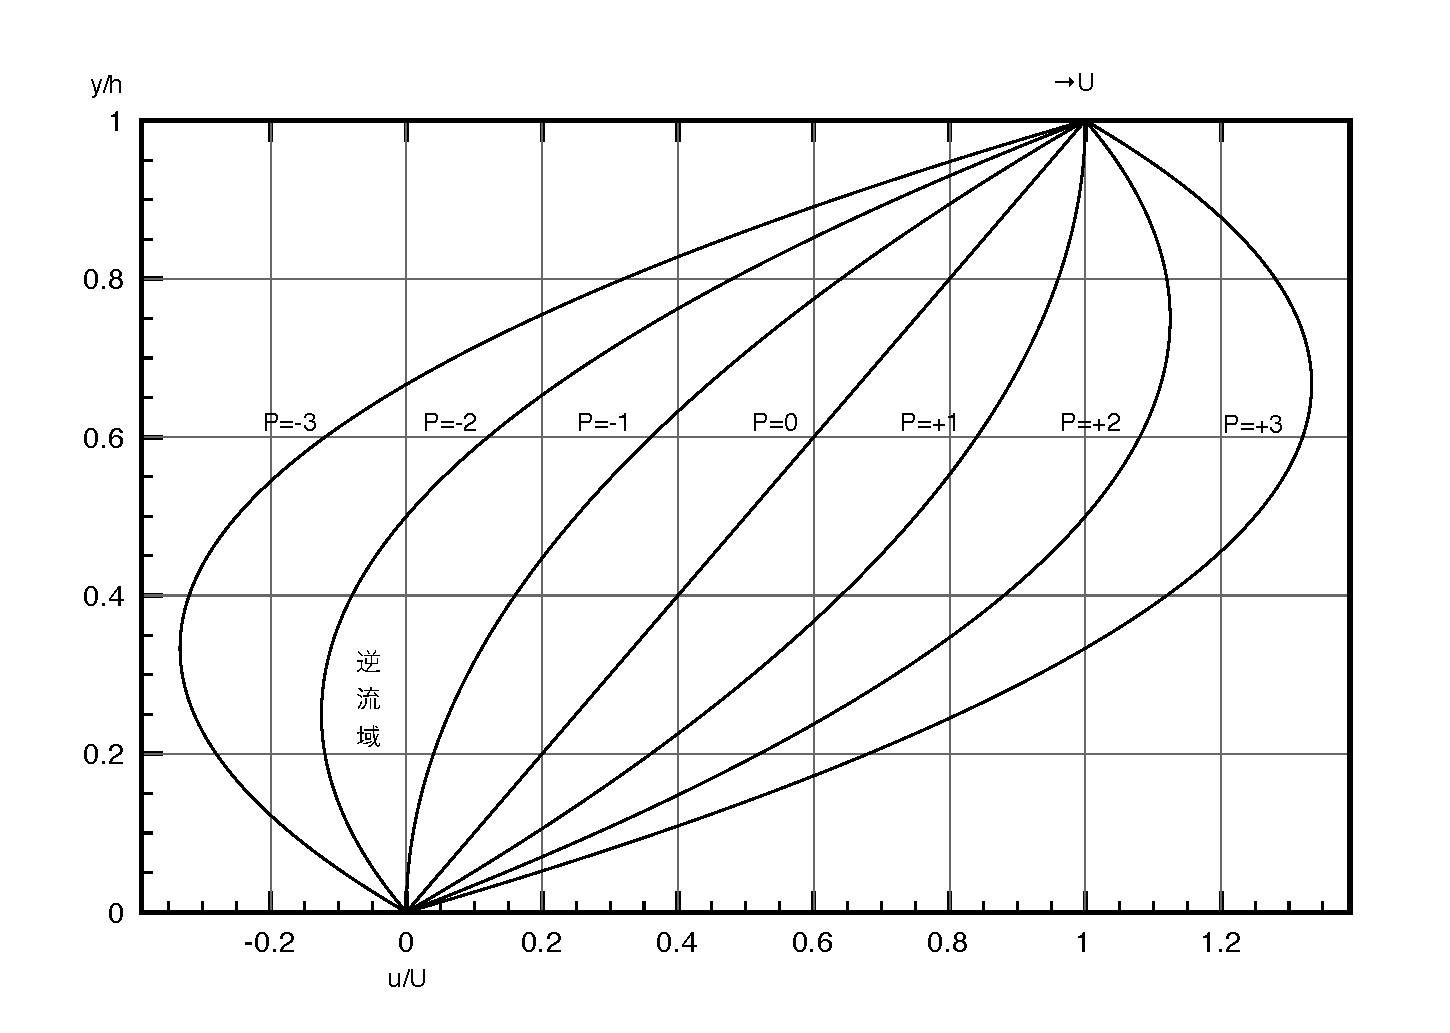
\includegraphics[width=12cm]{exact_solution.eps}
\caption{圧力勾配のある場合のCouette流}
\label{Fig.couetteG}
\end{figure}

\subsubsection{領域設定}
この例題は二次元問題なので,PPLT2D組込例題
クラスを使って計算する.
PPLT2Dクラスは辺長比が2:1の二次元空間を表現する.
$z$方向には3セルを設けており,\textbf{図\ref{Fig.couetteP}}に示すように,単純な周期境界条件を用いて二次元を近似している.
本計算では,$100\times50\times3$のセル分割とした.

コンフィギュレーションファイルの``Example"タグで``Parallel\_Plate\_2D"を指定する.
Couette流を再現するために,$x$軸方向に圧力勾配をかけた周期境界条件を設定し,$y=0$面は固定壁,$y=h$面はスライド($u=U$)壁とみなし,$z\pm$面には単純な周期境界条件を与える.

\begin{figure}[htbp]
\centering
\includegraphics[width=12cm, bb=0 0 646 405]{2Dcouette_model.png}
\caption{計算領域の設定}
\label{Fig.couetteP}
\end{figure}

\pagebreak
\subsubsection{計算環境}
本計算に利用した計算機環境とソフトウェアを\textbf{表\ref{tbl: 2dcouette env}}に示す.

\begin{table}[htdp]
\small
\caption{計算機環境および利用ソフトウェア}
\begin{center}
\begin{tabular}{ll}\toprule
Computer & eX. COMPUTER\\
CPU & Intel Core i7-950 (4 Cores/CPU)$\times$ 2\\
Clock & 3.07 GHz\\
Memory & 12GB \\
Cache & 8 MB(each CPU)\\
%Cache(3rd) & 4MB\\ 
OS & Linux ubuntu 2.6.32-25-generic\\ \hline
MPI & OpenMPI 1.4.3\\
V-Sphere & ver. 1.8.4\\
CBC & ver. 1.3.8\\
FlowBase & ver. 2.3.8\\ \hline
Compiler & Intel Compiler Composer XE(12.0) 2011.3.174 C++/Fortran\\
Compile Option & -O3\\
\bottomrule
\end{tabular}
\end{center}
\label{tbl: 2dcouette env}
\end{table}


%
\subsubsection{計算パラメータ}

計算に用いたパラメータ(\textbf{表\ref{Table.2Dcouette_param}}),流体の物性値(\textbf{表\ref{Table.2Dcouette_bussei}})などを示す.
\begin{table}[htbp]
\centering
\caption{計算に用いたパラメータ}
\label{Table.2Dcouette_param}
\begin{tabular}{llll}\toprule
$h$ &短辺の長さ &$1.0$ &[m]\\
$U$ &$y=h$の壁面の移動速度 & $1.0$ &[m/s]\\
$\Delta p$ &$x\pm$面間の圧力差($P=1$に相当) &$4.7052\times10^{-2}$ &[Pa]\\
$\nu $ & クーラン数 & 0.2& \\
\bottomrule
\end{tabular}
\end{table}

\begin{table}[htbp]
\centering
\caption{計算に用いた物性値}
\label{Table.2Dcouette_bussei}
\begin{tabular}{llll}\toprule
物性 &&物性値  & [単位]\\
\midrule
$\rho$ & 密度 & 1.1763 & [kg/m$^3$]\\
$\mu$  & 粘性係数 & 1.1763 $\times 10^{-2}$ &[Pa $\cdot$ s]\\
\bottomrule
\end{tabular}
\end{table}

\textbf{表\ref{Table.2Dcouette_param}},\textbf{表\ref{Table.2Dcouette_bussei}}から,レイノルズ数は,Re=$\rho U h/\mu=100$となる.
レイリーの問題から,時間$t$[s]の間に壁の影響が粘性を通じて及ぶ距離$\delta$[m]は,$\delta=\sqrt{t\nu}$.$\nu$は動粘性係数[m$^2$/s].無次元にすると$t^*=\delta^{*2}\cdot Re$となり,$\delta^*=1$,Re=100より,計算時間をt=100[-]と見積もった.

\paragraph{サンプリングの指定}
値のサンプリングは,$z=0, x=h$上の$y=0 \sim h$の範囲を分割してサンプリングする.今回の計算では,分割数を25とした.

\paragraph{外部境界条件}コンフィギュレーションファイルの中で,外部境界条件において,圧力勾配($P=+1$)をかける周期境界条件と,圧力勾配をかけない周期境界条件($z\pm$面)を設定する様子を示す.
{\small
\begin{program}
    <OuterBoundary>
      <Elem name="Basic_BCs">
        <Elem name="Wall" id="1">
            <Param dtype="REAL" name="Normal_X" value="0.0"/>
            <Param dtype="REAL" name="Normal_Y" value="0.0"/>
            <Param dtype="REAL" name="Normal_Z" value="0.0"/>
            <Param dtype="STRING" name="Specified_Type" value="Velocity"/>
            <Param dtype="STRING" name="Profile" value="Constant"/>
            <Param dtype="REAL" name="Specified_Value" value="0.0"/>
        </Elem>
        <Elem name="Wall" id="2">
            <Param dtype="REAL" name="Normal_X" value="1.0"/>
            <Param dtype="REAL" name="Normal_Y" value="0.0"/>
            <Param dtype="REAL" name="Normal_Z" value="0.0"/>
            <Param dtype="STRING" name="Specified_Type" value="Velocity"/>
            <Param dtype="STRING" name="Profile" value="Constant"/>
            <Param dtype="REAL" name="Specified_Value" value="1.0"/>
        </Elem>
        <Elem name="periodic" id="7" >
          <Param name="mode" dtype="string" value="simple_copy" />
        </Elem>
        <Elem name="periodic" id="8" >
          <Param name="mode" dtype="string" value="Directional" />
          <Param name="pressure_difference" dtype="REAL" value="0.047052" />
          <Param name="flow_direction" dtype="string" value="upstream" />
        </Elem>
        <Elem name="periodic" id="9" >
          <Param name="mode" dtype="string" value="Directional" />
          <Param name="pressure_difference" dtype="REAL" value="0.047052" />
          <Param name="flow_direction" dtype="string" value="downstream" />
        </Elem>
      </Elem>
	
      <Elem name="Face_BC">
        <Elem name="X_MINUS" id="8" comment="periodic_upstream">
          <Param name="Guide_Cell_ID" id="1" />
        </Elem>
        <Elem name="X_PLUS"  id="9" comment="periodic_downstream">
          <Param name="Guide_Cell_ID" id="1" />
        </Elem>
        <Elem name="Y_MINUS" id="1" comment="wall">
          <Param name="Guide_Cell_ID" id="600" />
        </Elem>
        <Elem name="Y_PLUS"  id="2" comment="slidewall">
          <Param name="Guide_Cell_ID" id="600" />
        </Elem>
        <Elem name="Z_MINUS" id="7" comment="periodic">
          <Param name="Guide_Cell_ID" id="1" />
        </Elem>
        <Elem name="Z_PLUS"  id="7" comment="periodic">
          <Param name="Guide_Cell_ID" id="1" />
        </Elem>
      </Elem>
    </OuterBoundary>
\end{program}
}

%
\subsubsection{計算結果と厳密解の比較}
\textbf{図\ref{Fig.couette_exact_100}}に,無次元圧力勾配$P=-3, -2, -1, 0, +1, +2, +3$の場合の,厳密解(実線)およびCBCの計算結果$u/U$(マーク)の値を比較した.CBCと厳密解の誤差は,厳密解の0.01\%以内に収まっており,よく一致しているといえる.


\begin{figure}[htbp]
\begin{center}
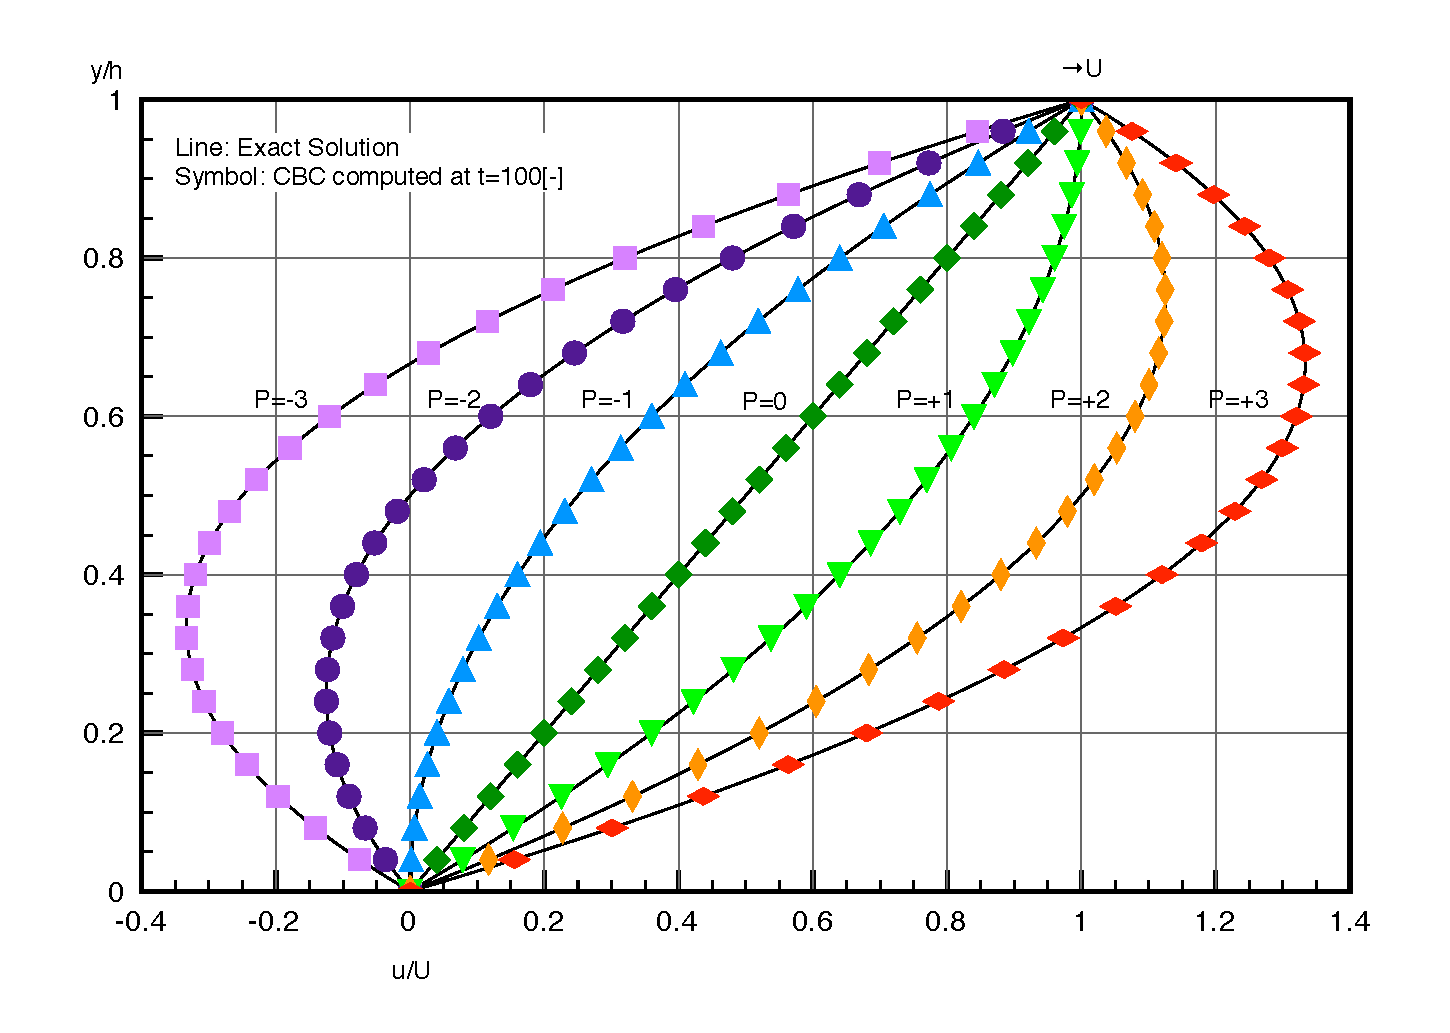
\includegraphics[width=14cm]{exact_100.eps}
\end{center}
\caption{圧力勾配のあるCouette流の速度分布(厳密解とCBCシミュレーションの比較)}
\label{Fig.couette_exact_100}
\end{figure}

%
\subsubsection{ファイルのメモ}
例題の提供ファイルの説明を以下に示す.\\
%\begin{quote}
\begin{tabularx}{180mm}{lclclX}
%\hspace{12em}\= \hspace{30em}\kill
example\CID{07480}2Dcouette & \CID{07530}&\CID{00718}&\CID{07530}&couette.xml & 圧力勾配$*:P=-3,\,-2,\,-1,\,0,\,1,\,2,\,3$の場合のコンフィギュレーションファイル\\
&\CID{07482}&&\CID{07514}&condition.txt & conditionファイル
\\
&\CID{07482}&&\CID{07514}&profiling.txt & 実行時性能測定結果ファイル\\
&\CID{07482}&&\CID{07514}&sample\_x=0.log& samplingファイル\\
&\CID{07482}&&\CID{07502}&history\_base.log&履歴ファイル\\
%&\CID{07482}&&\CID{07502}&(error\_P=+3.plot) & $P=+3$における解析解と厳密解との誤差.図\ref{Fig.couette.error} (\url{http://plot.micw.eu/})
%\\
%&\CID{07514}&\multicolumn{3}{l}{exact.f90} & 厳密解を計算するFortranコード\\
&\CID{07502}&\multicolumn{3}{l}{exact\_100.plot} &  厳密解と,$t=100[-]$における解析解の比較.\textbf{図\ref{Fig.couette_exact_100}}\\
& & &&&(\url{http://plot.micw.eu/})
\end{tabularx}
\\
\paragraph{conditionファイル内の無次元圧力勾配について}
condition.txtファイルの\lq\lq Outer Boundary Conditions\rq\rq セクションに,
周期境界条件に関連して,圧力差と圧力勾配の有次元値と無次元値が記載されている.
CBCではこの無次元化について,「圧力勾配のあるCouette流」に特有の\textbf{式(\ref{eq:P})}を使わず,通常Navier-Stokes方程式で使われる無次元化$p^*=p/(\rho U^2)$,$x^*=x/L$,$(dp/dx)^*=(dp/dx)\,L/(\rho U^2)$を用いている.そのため,圧力勾配$P=a$のcondition.txtファイルのPressure Gradientの無次元値が$a$と異なる値になっている.

具体的に,無次元圧力勾配$P=1$の場合を示すと,
{\small
\begin{verbatim}
	>> Outer Boundary Conditions

	      Set X- up as Periodic : (periodic_upstream)
       Guide Cell ID = 1 / Medium = 800
       Pressure Difference = 4.705200e-02 [Pa]    /  4.000000e-02 [-]
       Pressure Gradient   = 2.352600e-02 [Pa/m]  /  2.000000e-02 [-]

	      Set X+ up as Periodic : (periodic_downstream)
       Guide Cell ID = 1 / Medium = 800
       Pressure Difference = 4.705200e-02 [Pa]    /  4.000000e-02 [-]
       Pressure Gradient   = 2.352600e-02 [Pa/m]  /  2.000000e-02 [-]
\end{verbatim}
}

圧力勾配の無次元化は,\textbf{式(\ref{eq:P})}に従うと,
\[
P=\frac{h^2}{2\mu}\frac{1}{U}\left(-\frac{dp}{dx}\right)
  =\frac{1.0[m^2]}{2\times 1.1763\times10^{-2}[Pa\cdot s]\times 1.0[m \cdot s^{-1}]}\times 2.3526 \times 10^{-2}[Pa\cdot m^{-1}]
=1.0000[-]
\]
通常の無次元化を用いると,
\[
\left(\frac{dp}{dx}\right)^*=\frac{dp}{dx}\frac{L}{\rho U^2}
=2.3526 \times 10^{-2}[Pa\cdot m^{-1}]\times 
\frac{1.0[m]}{1.1763 \times 10^{-2}[Pa\cdot s] \times 1.0[m^2]}
=2.0000\times 10^{-2}[-]
\]
のようになる.

%\end{quote}

